%%%%%%%%%%%%%%%%%%%%%%%%%%%%%%%%%%%%%%%%%%%%%%%%%%%%%%%%%%%%%%%%%%%%%%%%%%%%%%%%%%%%%%%%%%%%%%%%%%%%%%%%%%%%%%%%%%%%%%%%%%%%%%%%%%%%%%%%%%%%%%%%%%%%%%%%%%%
% English manuscript generated from the English outline markdown.
%%%%%%%%%%%%%%%%%%%%%%%%%%%%%%%%%%%%%%%%%%%%%%%%%%%%%%%%%%%%%%%%%%%%%%%%%%%%%%%%%%%%%%%%%%%%%%%%%%%%%%%%%%%%%%%%%%%%%%%%%%%%%%%%%%%%%%%%%%%%%%%%%%%%%%%%%%%

\documentclass[utf8]{FrontiersinHarvard}
\usepackage{url,hyperref,lineno,microtype,subcaption}
\usepackage[onehalfspacing]{setspace}
\usepackage{tabularx,booktabs}
\usepackage{float}
\graphicspath{{figures/}}

\newcolumntype{Y}{>{\raggedright\arraybackslash}X}

\linenumbers

\def\keyFont{\fontsize{8}{11}\selectfont}
\def\firstAuthorLast{Shimizu {et~al.}}
\def\Authors{Yuki Shimizu\,$^{1,*}$, Midori Ban\,$^{2}$, Hideyuki Takahashi\,$^{3}$ and Hiroshi Ishiguro\,$^{1}$}
\def\Address{$^{1}$Department of Engineering Science, Osaka University, Osaka, Japan \\
$^{2}$Kyoto Tachibana University, Kyoto, Japan \\
$^{3}$Faculty of Science and Engineering, Otemon Gakuin University, Osaka, Japan}
\def\corrAuthor{Yuki Shimizu}
\def\corrEmail{simizu.yuki@irl.sys.es.osaka-u.ac.jp}

\begin{document}
\onecolumn
\firstpage{1}

\title[Robot-expressed approach-avoidance conflict]{Effects of Observing a Robot Expressing Approach-Avoidance Conflict on Observers' Self-Evaluations of Personal Courage}

\author[\firstAuthorLast ]{\Authors}
\address{}
\correspondance{}
\extraAuth{}

\maketitle

\begin{abstract}
This study examined whether a robot's externalization of approach-avoidance conflict before action influences observers' self-evaluations of personal courage. Personal courage involves not only moving toward a valued action but also the internal state of experiencing fear or hesitation before acting. In this study, speech bubbles were displayed near the head of a cylindrical robot using projection mapping, and approach and avoidance motives were presented in a scene in which the robot confronted littering in a park.

Study 1 compared conflict and no-conflict conditions, as well as sequential and simultaneous presentation methods, to examine whether a robot expressing approach-avoidance conflict was perceived as courageous. Study 2 used the simultaneous presentation selected in Study 1 and examined how the presence or absence of conflict and admonishing behavior influenced post-stimulus self-evaluations of personal courage in relation to observers' pre-existing courage tendency.

In Study 1, the conflict condition produced higher courage ratings and conflict ratings than the no-conflict condition, confirming that the presented internal state was perceived as conflict. In Study 2, the interaction between pre-existing courage tendency and conflict was significant: participants in the low-courage group tended to show higher self-evaluations in the conflict condition, whereas participants in the high-courage group showed lower self-evaluations in the conflict condition. In contrast, the presence or absence of admonishing behavior showed no clear effect. These findings suggest that visually externalizing approach-avoidance conflict through a robot may influence observers' self-evaluations of personal courage. However, this influence may not be uniform and may differ depending on observers' pre-existing courage tendency.

{\fontsize{8}{11}\selectfont\sloppy\noindent\textbf{Keywords:} personal courage, approach-avoidance conflict, observational learning, human-robot interaction, internal state, robot expression, social modeling\par}
\end{abstract}

\section{Introduction}

In everyday life, people sometimes need to move toward valued actions even in situations that involve fear or anxiety. In this study, we refer to the capacity to move toward such actions as personal courage. Courage has been conceptualized not as the absence of fear but as moving toward meaningful action in the presence of fear \citep{rachman1984,woodard2007}. Personal courage is important because it allows the difficulty of an action to be understood in relation to the actor's own context. Pury et al. distinguished between general courage, which is evaluated as courageous by most people, and personal courage, which is courageous in light of a person's life context and personal constraints \citep{pury2007}. From this perspective, a child with a learning disability going to school on the day of a major test, or a person wrapping Christmas presents for the first time after being unable to do so for many years because of a history of PTSD, can be understood as actions involving high fear and difficulty in that person's context \citep{pury2007}. Furthermore, actions such as speaking up, seeking help, or pointing out a problem may be valuable for the person or others, but they also involve social and psychological risks such as lowered evaluation and rejection. These actions are therefore meaningful targets for investigation from the perspective of personal courage \citep{howard2017,vogel2007,milliken2003}.

However, people do not always act even when they recognize that an action is valuable. For example, expressing an opinion in front of others often involves anxiety about how one will be evaluated \citep{watson1969,dickerson2004}. Consulting others or seeking help can also involve concern about being viewed negatively \citep{vogel2007}. In workplaces, many employees report having noticed problems or concerns but not communicated them to supervisors, and the main reasons include fear of being viewed negatively or damaging important relationships \citep{milliken2003}. In other words, speaking up and seeking help can be beneficial for oneself and others, yet they involve social and psychological risks such as lowered evaluation, damaged relationships, reduced status, and loss of self-image. Therefore, supporting personal courage requires more than helping people understand that an action is valuable; it also requires supporting the process of moving toward action while perceiving risk.

As one way to support this process, the present study focuses on observational learning. Observational learning refers to learning in which observing another person's behavior or success increases one's expectation that ``I may be able to do it too'' \citep{bandura1977}. The effectiveness of observational learning was first demonstrated in learning actions that are visible from the outside. For example, children who were afraid of swimming showed better skill outcomes after observing same-age models swimming \citep{weiss1998}. In studies of sit-to-stand and stand-to-sit action observation, observers' sensorimotor systems respond, and action observation itself can activate motor representations \citep{chaisaen2020}. At the same time, observational learning can also involve psychological aspects such as effort and persistence, not only externally visible movements. Schunk and Hanson showed that observing peer models affects children's self-efficacy and achievement behavior \citep{schunk1985}. In addition, infants who observed an adult struggling to achieve a goal made more attempts on a subsequent difficult task than infants who observed an adult easily succeeding \citep{leonard2017}. These findings suggest that observing others facing difficulty can support observers' sense that they too can try and can encourage persistence.

The purpose of this study is to clarify how presenting personal courage as an object of observational learning affects observers' self-evaluations of their own personal courage. In personal courage, not only ``what was done'' but also ``how frightening it was'' and ``what kind of hesitation was involved'' are important \citep{pury2007}. However, when a human model is used, it is difficult to present fear or conflict before action in the same form and intensity across conditions. Therefore, in this study, we used a robot to express a state in which the motivation to move toward a valued action and the motivation to avoid risk or disadvantage coexist as approach-avoidance conflict, and we examined whether observing this state influences observers' self-evaluations of personal courage.

We conducted two studies. Study 1 clarified what kind of robot expression is perceived as a ``courage-evoking action.'' Specifically, we examined whether a robot expressing approach-avoidance conflict is perceived as more courageous than a robot not expressing conflict, and we assessed the validity of the stimulus to be used in Study 2. Study 2 examined whether observing the robot that was confirmed in Study 1 to be perceived as courageous influences observers' self-evaluations of personal courage. In addition, to separate the effect of presenting approach-avoidance conflict from the observational effect of seeing a valued action, we independently manipulated the presence or absence of conflict and the presence or absence of action. Through this design, the present study provides insight into the meaning of presenting not only action itself but also the internal state before action when personal courage is treated as a target of observational learning. It also provides methodological implications for using robots to visualize internal states that are difficult to observe from the outside and to support observational learning related to courage.

\section{Related Work}

\subsection{Personal Courage and Internal States Before Action}

Research on courage has treated courage not as the absence of fear but as moving toward action while experiencing fear. Rachman argued that even people with strong fear can perform courageous acts \citep{rachman1984}. Norton and Weiss examined the relationship between behavioral approach and courage in a fear-eliciting situation \citep{norton2009}. Woodard and Pury also conceptualized courage as a construct involving action for a meaningful purpose in a situation involving threat or fear \citep{woodard2007}. These studies provide a basis for understanding courage not as mere risk preference or low fear but as approach behavior in the presence of fear.

Among these studies, Pury et al. distinguished between general courage, which is evaluated as courageous by most people, and personal courage, which is courageous in light of a person's life context and personal constraints \citep{pury2007}. Highly personal courageous actions are characterized by fear, difficulty, and personal constraints. From this distinction, the same action may or may not be courageous depending on what kinds of fear or difficulty the actor experienced. Therefore, research on personal courage needs to consider not only externally visible behavior but also the internal states preceding that behavior.

Recent models explaining the mechanisms by which courage emerges also focus on these internal states before action. Chowkase et al. describe courage as a sequence involving situation perception, evaluation of value or meaning, evaluation of action feasibility, and action decision \citep{chowkase2024}. In this process, reasons to move toward a valued action and reasons to avoid risks or disadvantages associated with the action may coexist. This can be understood as approach-avoidance conflict, in which approach and avoidance motives operate simultaneously \citep{lewin1931,miller1944}. However, these studies clarify the definition and process of courage; they do not directly examine whether observing another agent's internal state changes observers' self-evaluations of personal courage.

\subsection{Observational Learning and Dependence on Observers' Prior Characteristics}

Research on observational learning has shown that observing others' behavior and its outcomes can change observers' behavior, motivation, and self-efficacy. Bandura positioned vicarious experience as one source of self-efficacy and argued that observing another person succeed at a task can influence the expectation that ``I can do it too'' \citep{bandura1977}. Schunk and Hanson showed that observing peer models affects children's self-efficacy and achievement behavior \citep{schunk1985}. These studies suggest that observing others act can influence the cognition that observers themselves can also perform the action.

The effect of a model can also differ depending on the state in which the model acts. Schunk et al. compared mastery models who succeeded easily from the beginning with coping models who showed difficulty and gradually coped with it, and found that observing coping models increased self-efficacy and task performance \citep{schunk1987}. Schunk and Hanson also showed that models who cope while showing difficulty and negative affect influence learning self-efficacy \citep{schunk1989}. Leonard et al. showed that infants who observed an adult persisting in an attempt to achieve a goal made more attempts on a subsequent difficult task than infants who observed an adult easily succeed \citep{leonard2017}. These findings suggest that observing a process involving difficulty and effort can support observers' self-efficacy and persistence.

At the same time, the same model may be received differently depending on observers' prior characteristics. Braaksma et al. showed that similarity between model and observer and the model's level of expertise are important in observational learning \citep{braaksma2002}. Lucas et al. showed that people tend to rely on others' judgments and behavior as cues when a task is difficult, whereas people with high self-efficacy are less susceptible to such social influence \citep{lucas2006}. These findings indicate that, when using observational learning, it is necessary to consider not only the model's characteristics but also observers' prior characteristics, which influence how the model is received. Therefore, the present study also considers observers' prior characteristics when examining the effect of a robot's conflict expression.

\subsection{Modeling by Robots and Artificial Agents}

Models in observational learning are not limited to humans. Studies using artificial agents and avatars have shown that visually present agents and avatars similar to the self can influence observers' attitudes, self-efficacy, and subsequent behavior \citep{rosenberg2008,fox2009}. Research on social robots has also shown that people can treat robots as social models and engage in modeling based on their behavior and social roles \citep{xu2023}. It has also been reported that the way a robot encourages participants influences the way participants subsequently encourage others \citep{higashino2023}.

These studies indicate that robots and artificial agents can function as social models that influence observers. However, the studies reviewed here targeted attitudes, self-efficacy, movement, and encouragement behavior, not personal courage itself. To the extent reviewed in this manuscript, few studies have explicitly presented what kind of fear or conflict a model has before action and examined how observing it influences observers' self-evaluations of personal courage. Therefore, using a robot to present internal states related to personal courage in an observable form extends existing modeling research.

\subsection{Externalizing Internal States Through Robots}

The experimental reason for using a robot in this study is that visual expressions, in addition to behavior and speech, can be more easily controlled across conditions. With a human model, observers can infer internal states from facial expressions, voice, silence, or self-disclosure. However, to present the presence or absence of fear, hesitation, approach motives, and avoidance motives in the same scenario and in a comparable form across conditions, an artificial medium is more suitable. Therefore, in this study, we used speech-bubble expressions in addition to the robot's movement and speech, and presented the robot as a stimulus in which internal states were externalized.

Regarding speech-bubble expressions, Nitada et al. proposed a method in which a speech bubble is displayed near a robot's head in a video-conferencing situation, with the user's face drawn inside the bubble \citep{nitada2021}. They found that the speech-bubble condition increased the sense that the robot was looking at the user. This study suggests that speech bubbles can function as a means of visually representing the robot's attention or mental focus. However, that study addressed the direction of attention, not the conflict between approach and avoidance motives related to courage.

Taken together, prior studies have shown that personal courage involves actions accompanied by fear or difficulty, that observational learning can influence self-efficacy and perceived action possibility, and that robots and artificial agents can function as social models. However, to the extent reviewed in this manuscript, research has not sufficiently examined whether externalizing, through a robot, internal states before action related to personal courage, especially conflict between approach and avoidance motives, affects observers' self-evaluations of personal courage. The present study focuses on this unexplored issue and examines how observing a robot expressing approach-avoidance conflict relates to observers' self-evaluations of personal courage.

\section{Design of the Video Stimuli}

\subsection{Robot and Projection Environment}

The robot used in this study had the same body as the switch-based robot interface proposed by Omichi et al. (ICSR 2025). This robot has a cylindrical body, and an agent with a face emerges from inside the body and speaks \citep{omichi2026}.

This study examined whether presenting the robot's internal state before action through speech bubbles influences observers' self-evaluations of personal courage. Therefore, it was necessary to minimize interpretive variability arising from the robot's appearance or bodily movements. Unlike humanoid robots, this robot does not involve complex facial expressions or limb movements; its main expressions are limited to face presentation and speech. Therefore, we considered it suitable as a stimulus medium for presenting approach motives, avoidance motives, and the presence or absence of admonishing speech in a relatively controlled manner. For the admonishing speech, prerecorded audio was used and played by the experimenter through keyboard operation.

In the video stimuli, the robot was filmed so that it appeared in the lower-right corner of the frame, and the robot's internal state was displayed as a speech bubble projected by a projector onto the wall behind the robot. The speech bubble was positioned so that it appeared near the robot's head and was used not as the robot's speech but as a visual expression of the internal state before action.

\subsection{Stimulus Scenario}

In this study, we used video stimuli depicting a scene in which a robot sees a person littering in a park. Littering in a park is easily understood as a violation of shared norms in a public space. Indeed, littering has been used as a representative task for examining the effects of descriptive and injunctive norms \citep{cialdini1990}. Observational research in public spaces has also shown that the presence of existing litter increases littering, whereas the availability of trash bins reduces it. Thus, littering is positioned as an everyday norm violation that is affected by environmental and normative cues \citep{schultz2013}. In addition, cues of disorder such as litter and graffiti can induce other norm violations \citep{keizer2008}. Therefore, admonishing the person in this scene has value in terms of keeping the park clean, creating an opportunity for the person to stop littering, and reaffirming the norm that littering is unacceptable. At the same time, admonishing a stranger involves social and psychological risks such as being yelled at, ignored, or viewed negatively. Littering in a park has also been used as a stimulus scenario in prior research on social control behavior and has some validity as a scene involving intervention in a stranger's norm violation \citep{chekroun2002}. Field research has further shown that sanctions against strangers' norm violations include not only direct admonition but also indirect methods, and that direct admonition can involve costs such as the possibility of retaliation \citep{balafoutas2014}. Research on social courage has identified moving toward valued action while facing interpersonal risk as an important feature \citep{howard2017}. Therefore, admonishing littering in a park is suitable as a stimulus scenario for examining personal courage because it involves both valued action and interpersonal risk, and it can elicit hesitation or conflict for the actor, even though it is not a situation involving extremely high physical danger.

An example of the scenario description in the stimulus is shown in Figure~\ref{fig:scene}.

\begin{figure}[htbp]
\centering
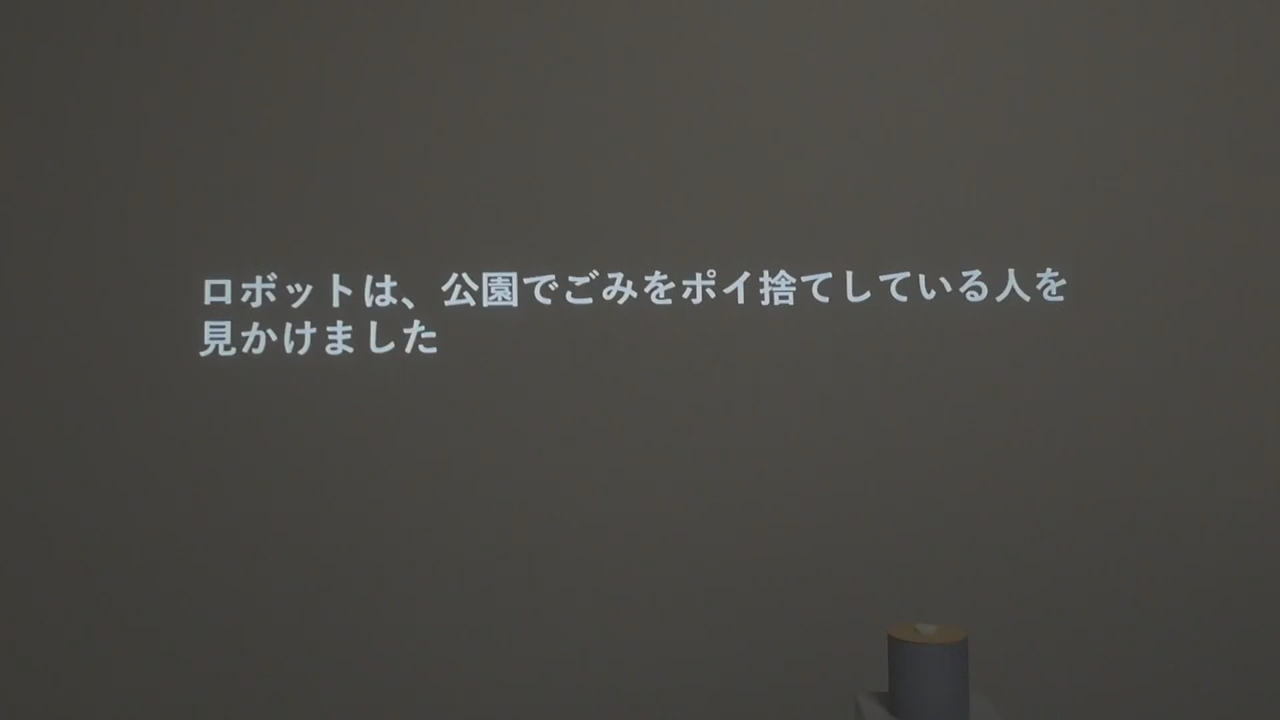
\includegraphics[width=0.86\linewidth]{fig1_scene.png}
\caption{Example of the scenario description in the video stimulus. Text presentation of the situation in which the robot sees a person littering in a park.}
\label{fig:scene}
\end{figure}

\subsection{Common Structure of the Video Stimuli}

The video stimuli did not present the park scene itself as live-action footage; instead, the scene was constructed using a textual scenario description and speech-bubble expressions. At the beginning of the video, the following scenario description was presented: ``The robot saw a person littering in a park.'' The robot then showed situation recognition in the speech bubble, such as ``Oh, there is a person littering,'' followed by cognition indicating that the situation required admonition. The subsequent presentation of motives and the presence or absence of admonishing speech were manipulated according to the conditions in each study. All videos were created at a resolution of 1280 x 720 pixels. The videos in Study 1 were approximately 50--54 seconds long, and the videos in Study 2 were approximately 49--50 seconds long.

\subsection{Approach Motives and Avoidance Motives}

In this study, reasons for moving toward a valued action were defined as approach motives, and reasons for wanting to avoid the risks or disadvantages associated with the action were defined as avoidance motives. The specific motive statements are shown in Table~\ref{tab:motives}. The approach motives indicated the possibility that desirable outcomes would result from admonishing behavior, whereas the avoidance motives indicated social and psychological risks that could result from admonishing behavior. By combining these approach and avoidance motives, the study expressed a state in which reasons for moving toward a valued action and reasons for avoiding that action coexist. This state is positioned as approach-avoidance conflict, in which approach and avoidance motives operate simultaneously \citep{lewin1931,miller1944}.

\begin{table}[htbp]
\centering
\small
\caption{Motive statements used in the video stimuli.}
\label{tab:motives}
\begin{tabularx}{\linewidth}{Y Y Y}
\toprule
Type of motive & Motive statement & Content \\
\midrule
Approach motive & ``If I warn them, the park might become cleaner.'' & Possibility that admonishing behavior improves the public space \\
Approach motive & ``If I warn them, it might prompt that person to stop littering.'' & Possibility that admonishing behavior changes the other person's behavior \\
Avoidance motive & ``I would hate it if they yelled at me after I warned them.'' & Risk of receiving an aggressive response from the other person because of admonishing behavior \\
Avoidance motive & ``Even if I warn them, they might ignore me and not take me seriously.'' & Risk that the admonition is not accepted and is ignored \\
\bottomrule
\end{tabularx}
\end{table}

An example in which the approach and avoidance motives were presented simultaneously is shown in Figure~\ref{fig:approach_avoidance}.

\begin{figure}[htbp]
\centering
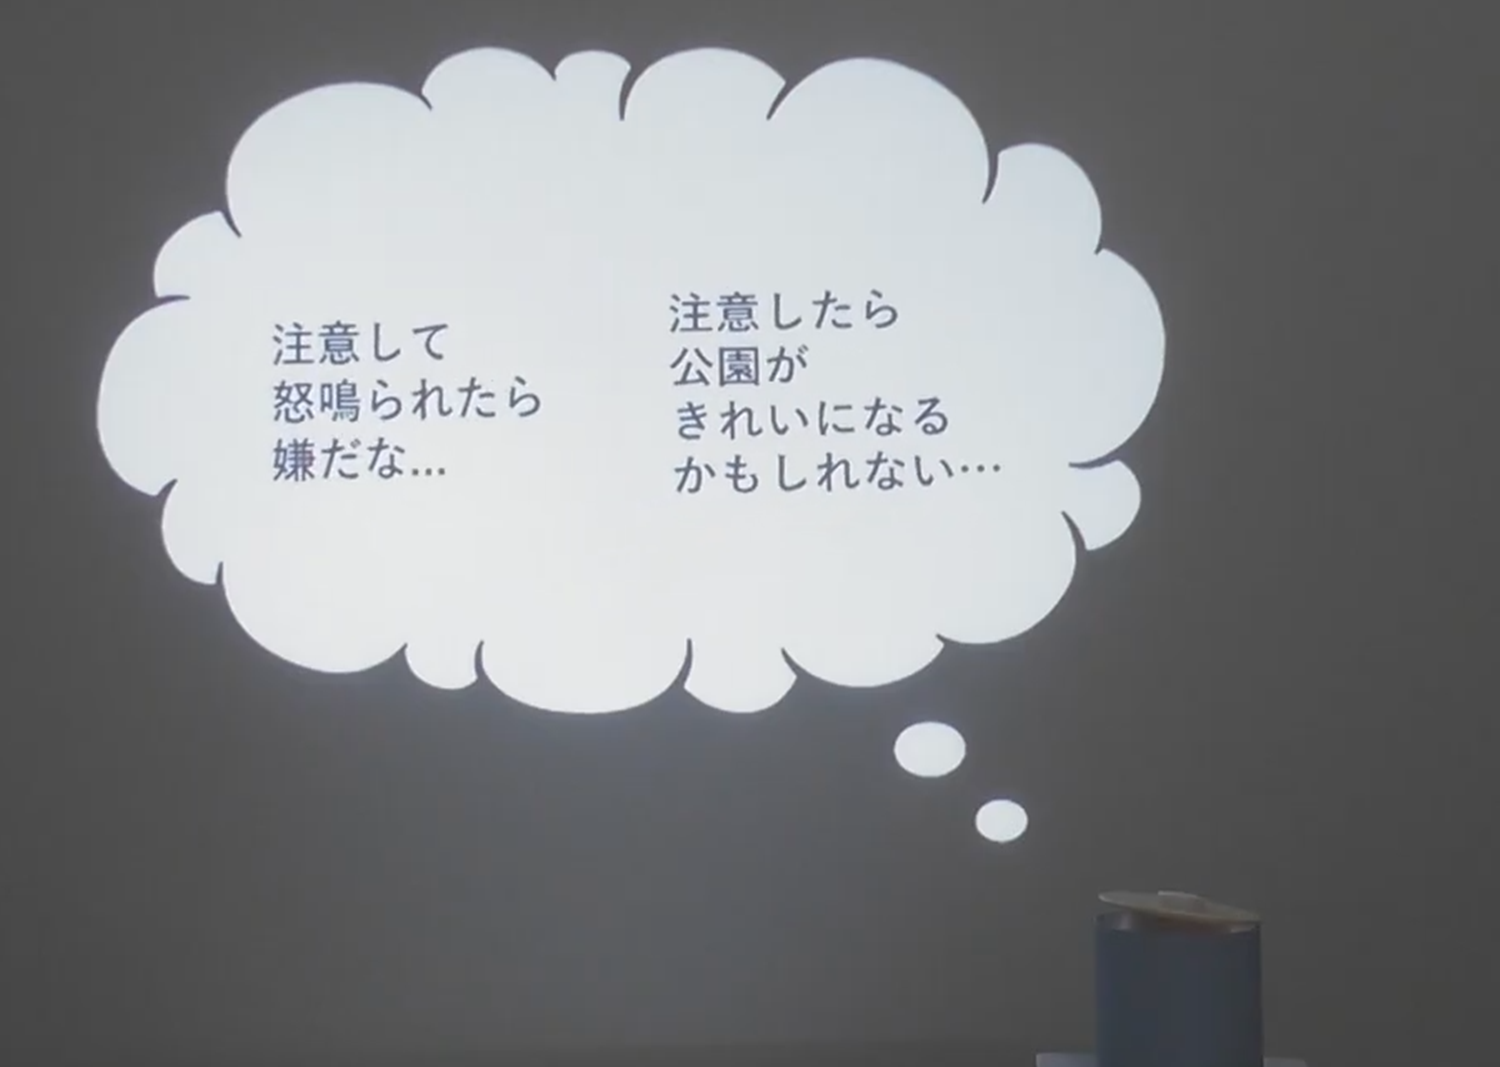
\includegraphics[width=0.86\linewidth]{fig2_conflict_large_text.png}
\caption{Example of simultaneous presentation of approach and avoidance motives. Simultaneous display of a desirable consequence of admonishing and a concern about admonishing.}
\label{fig:approach_avoidance}
\end{figure}

Through this common design, the present study presented internal states before action in a form that observers could visually understand. The details of the condition manipulations in each study are described in the respective method sections.

\section{Study 1: Is a Robot Expressing Approach-Avoidance Conflict Perceived as Courageous?}

\subsection{Purpose}

The purpose of Study 1 was to examine whether the presentation to be used in Study 2 would be perceived as courageous. Specifically, we examined whether a robot expressing approach-avoidance conflict as an internal state would be perceived as more courageous than a robot not expressing conflict. We also used conflict ratings to confirm whether the presented internal state was perceived as approach-avoidance conflict and explored which presentation method should be selected for Study 2.

Approach-avoidance conflict is described as a state in which approach and avoidance motives operate simultaneously \citep{lewin1931,miller1944}. At the same time, the experience of conflict may also occur as temporal fluctuation. Therefore, in Study 1, we considered two candidate methods: sequential presentation, in which approach and avoidance motives were presented in sequence, and simultaneous presentation, in which both motives were presented at the same time. In Study 1, courage ratings were prioritized, and if no difference was found, conflict ratings were used as a reference for selecting the presentation method for Study 2.

Based on this reasoning, we predicted that the conflict condition would produce higher robot courage ratings than the no-conflict condition. As a manipulation check, we also predicted that the conflict condition would produce higher conflict ratings than the no-conflict condition. The comparison between sequential and simultaneous presentation was exploratory, with the aim of examining which method would be perceived as more courageous.

\subsection{Method}

\subsubsection{Conditions}

Study 1 used a within-participant design with conflict and presentation method as factors. Conflict had two levels: no conflict and conflict. Presentation method had two levels: sequential presentation and simultaneous presentation. To avoid confounding the effect of the presence or absence of final action, all conditions in Study 1 presented the robot performing the admonishing action.

In the stimulus videos, after the robot saw a person littering in a park, it showed situation recognition and motives through a speech bubble. In the conflict condition, approach and avoidance motives were presented; in the no-conflict condition, only approach motives were presented. In the simultaneous presentation condition, approach and avoidance motives were presented simultaneously and alternately enlarged and reduced. In the sequential presentation condition, the two motives were presented in sequence. Finally, in all conditions, the robot said, ``Excuse me, this is not a place to throw away trash.''

\begin{table}[htbp]
\centering
\scriptsize
\caption{Study 1 conditions.}
\label{tab:study1_conditions}
\begin{tabularx}{\linewidth}{Y Y Y Y Y}
\toprule
Study 1 condition & Internal-state content & Motive statements used & Presentation method & Final admonishing speech \\
\midrule
No conflict, sequential presentation & Approach motives only & Approach motives: ``If I warn them, the park might become cleaner''; ``If I warn them, it might prompt that person to stop littering'' & Approach motives presented in sequence & Present \\
No conflict, simultaneous presentation & Approach motives only & Approach motives: ``If I warn them, the park might become cleaner''; ``If I warn them, it might prompt that person to stop littering'' & Multiple approach motives presented simultaneously and alternately emphasized & Present \\
Conflict, sequential presentation & Approach and avoidance motives & Approach motives: ``If I warn them, the park might become cleaner''; ``If I warn them, it might prompt that person to stop littering'' / Avoidance motives: ``I would hate it if they yelled at me after I warned them''; ``Even if I warn them, they might ignore me and not take me seriously'' & Approach and avoidance motives presented in sequence & Present \\
Conflict, simultaneous presentation & Approach and avoidance motives & Approach motives: ``If I warn them, the park might become cleaner''; ``If I warn them, it might prompt that person to stop littering'' / Avoidance motives: ``I would hate it if they yelled at me after I warned them''; ``Even if I warn them, they might ignore me and not take me seriously'' & Approach and avoidance motives presented simultaneously and alternately emphasized & Present \\
\bottomrule
\end{tabularx}
\end{table}

Representative frames related to the presentation methods in the conflict conditions of Study 1 are shown in Figure~\ref{fig:study1-conflict-presentation}. In Figure~\ref{fig:study1-conflict-presentation}, the scenario description, situation recognition, and cognition indicating that the situation required admonition are omitted; only the portions presenting the approach and avoidance motives are shown. In the sequential presentation condition, the avoidance motive ``I would hate it if they yelled at me after I warned them'' and the approach motive ``If I warn them, the park might become cleaner'' were presented in separate frames in sequence. In the simultaneous presentation condition, the same avoidance and approach motives were presented simultaneously within a single speech bubble and alternately emphasized.

\begin{figure}[htbp]
\centering
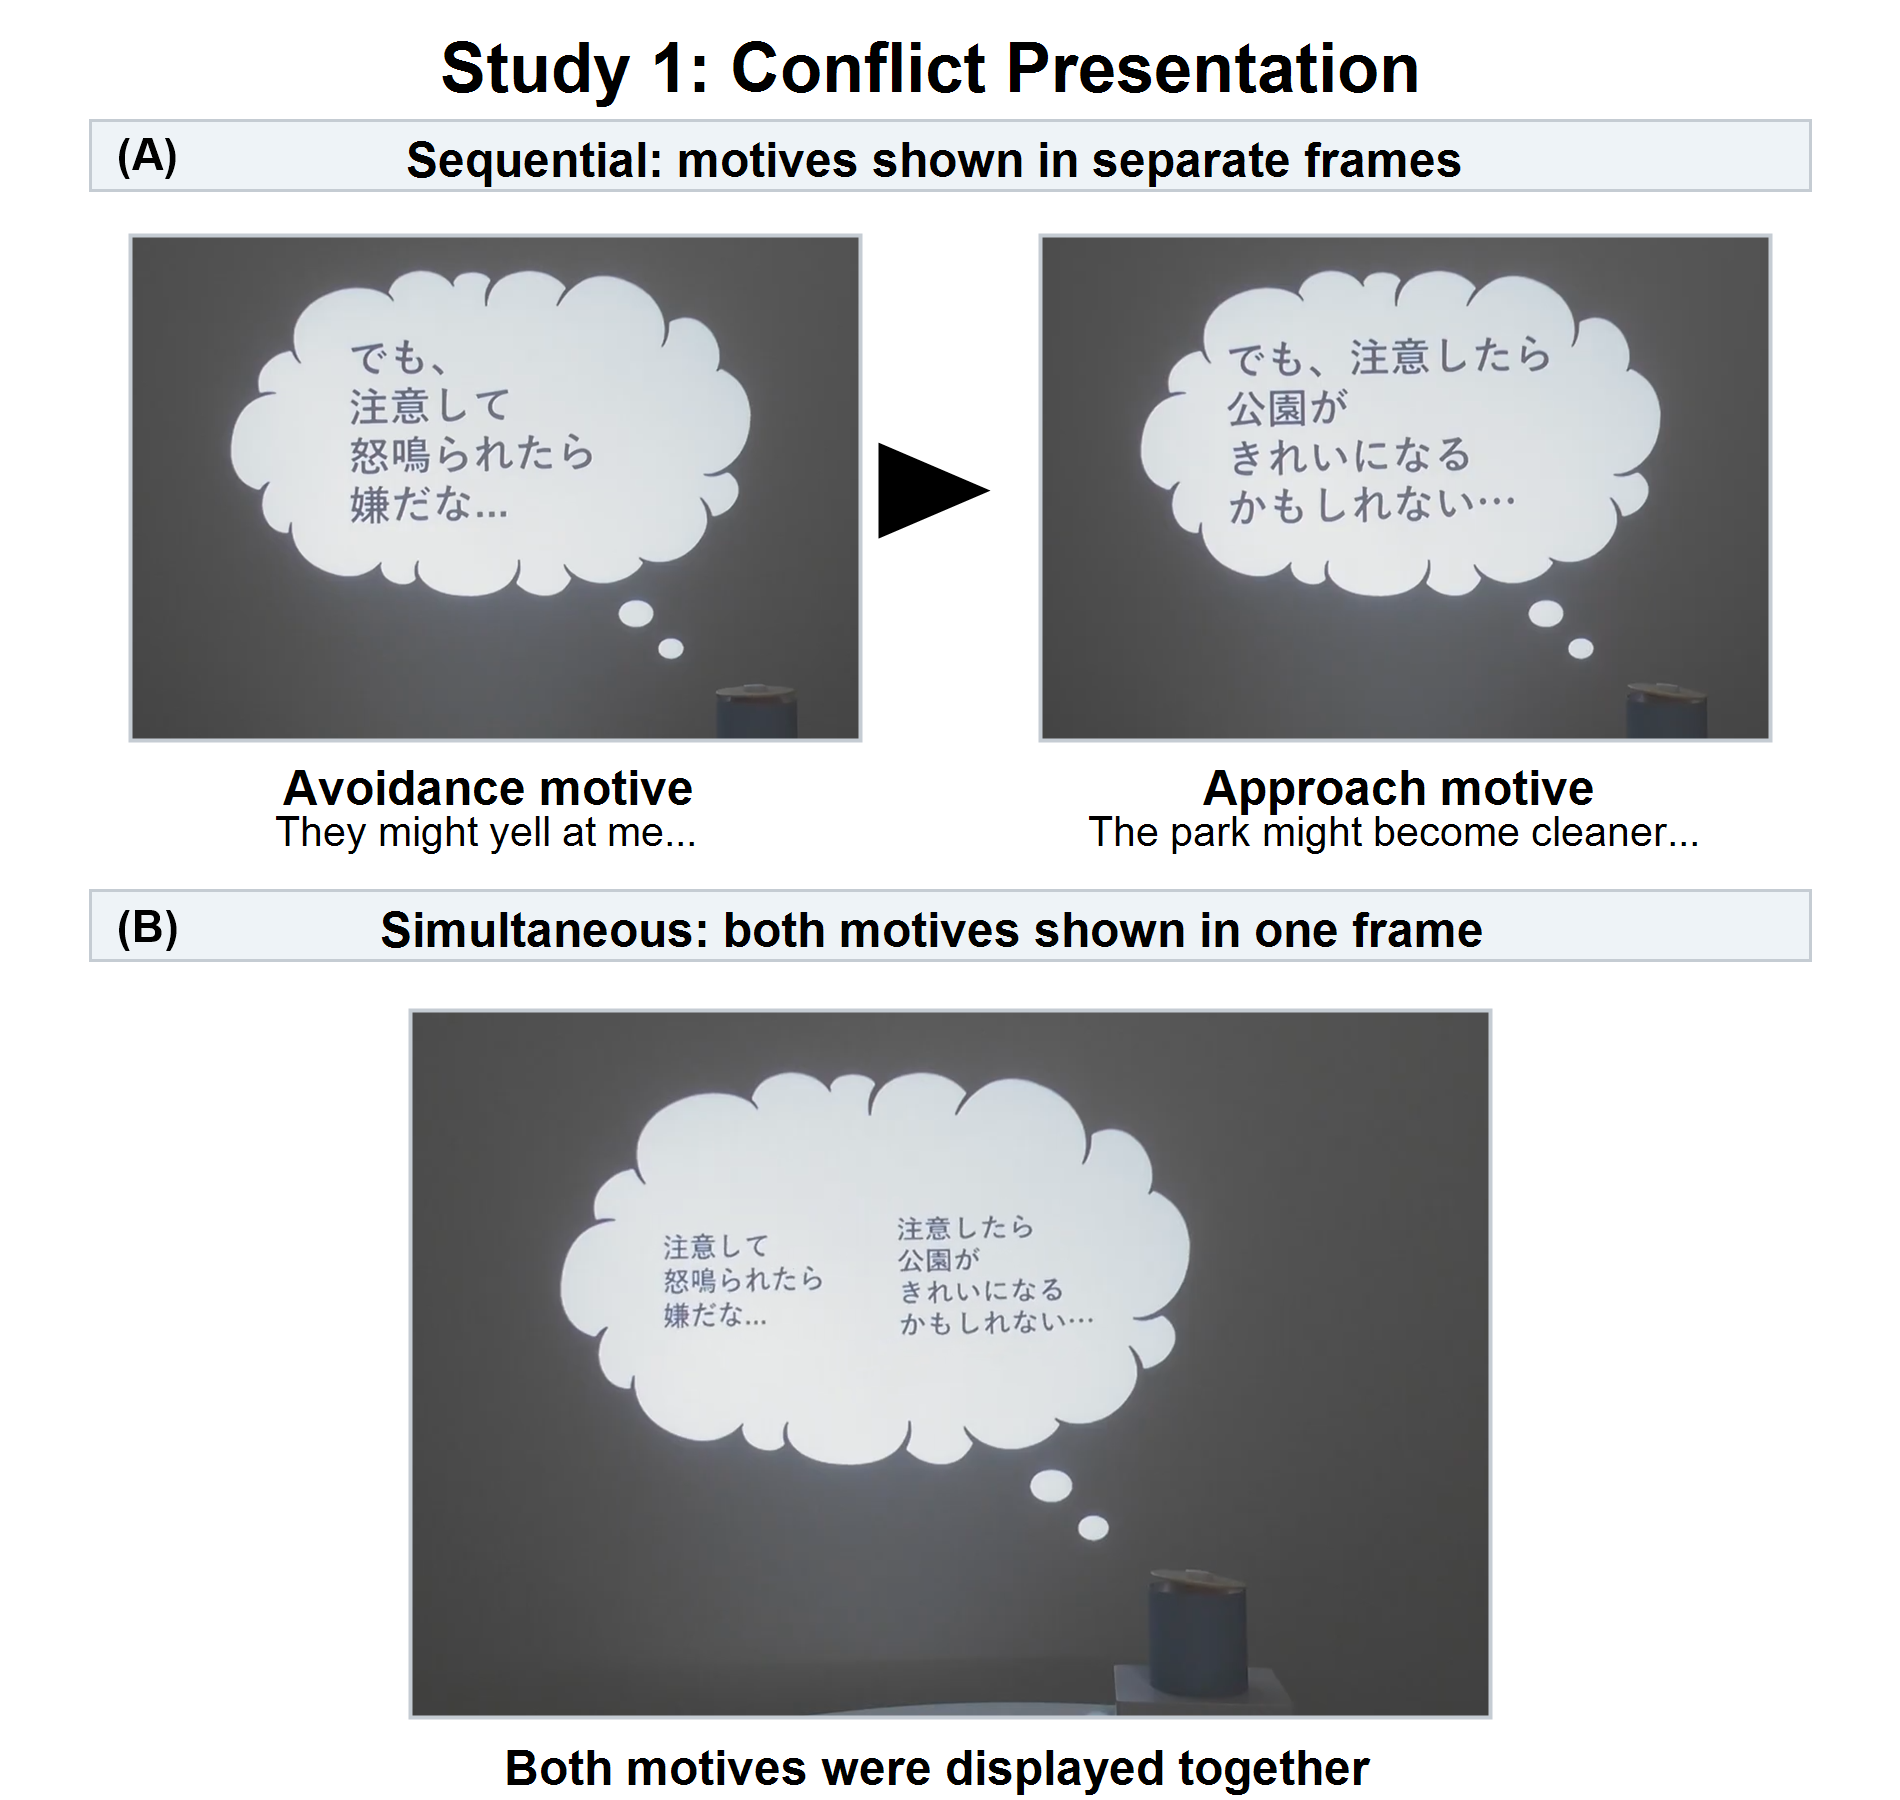
\includegraphics[width=\linewidth]{fig_study1_stimulus_flow.png}
\caption{Comparison of conflict presentation methods in Study 1. (A) In the sequential presentation condition, the avoidance and approach motives were shown in separate frames. (B) In the simultaneous presentation condition, both motives were shown within a single frame.}
\label{fig:study1-conflict-presentation}
\end{figure}

\subsubsection{Measurement}

The dependent variables were robot courage ratings and conflict ratings. Each rating was obtained on a 7-point scale after participants observed each video, and the mean of the items was used as the score. Courage ratings were created by modifying the six items of the Japanese version of the Courage Measure (CM-J) for rating the robot \citep{shimotsukasa2023}. The CM-J is a scale that measures the tendency to act despite fear or anxiety, and its reliability and validity have been confirmed \citep{shimotsukasa2023}. In Study 1, to measure the extent to which the robot appeared courageous rather than the observer's own courage, the subject of each item was changed to ``This robot,'' and item endings were changed to observational rating expressions such as ``appeared to'' and ``was.'' In the analysis, the mean of the six items was used as the courage rating score.

\begin{table}[htbp]
\centering
\small
\caption{Courage-rating items.}
\label{tab:courage_items}
\begin{tabularx}{\linewidth}{cY}
\toprule
Item & Courage-rating item \\
\midrule
1 & This robot appeared to confront its own fear. \\
2 & This robot appeared not to run away until it did what it had to do, even if it felt strong fear. \\
3 & This robot did something even though it seemed dangerous. \\
4 & This robot took action or confronted the situation anyway, even though it had some worry or anxiety. \\
5 & This robot confronted something frightening when there was an important reason to confront it. \\
6 & This robot appeared not to back down, even when something threatened it. \\
\bottomrule
\end{tabularx}
\end{table}

Conflict ratings were measured using original items to assess the extent to which the robot appeared to waver between approach and avoidance motives. In creating the items, based on the definition of approach-avoidance conflict \citep{lewin1931,miller1944}, we verbalized observable aspects of approach-avoidance conflict: wanting to do the thing in front of oneself but hesitating because of fear, having hesitation or fluctuation in action, having mixed feelings of wanting and not wanting to act, and being unable to decide one's action. In the analysis, the mean of the following four items was used as the conflict rating score. In addition, to confirm whether ratings based on these four items corresponded to a direct judgment of conflict, we also obtained a direct item: ``This robot appeared to be experiencing conflict.''

\begin{table}[htbp]
\centering
\small
\caption{Conflict-rating items.}
\label{tab:conflict_items}
\begin{tabularx}{\linewidth}{cY}
\toprule
Item & Conflict-rating item \\
\midrule
1 & This robot appeared to want to do what was in front of it but to hesitate because of fear. \\
2 & This robot appeared to have hesitation or fluctuation in its own action. \\
3 & This robot appeared to have mixed feelings of wanting and not wanting to act. \\
4 & This robot appeared unable to decide its own action. \\
\bottomrule
\end{tabularx}
\end{table}

\subsubsection{Procedure}

Study 1 was conducted on Yahoo! Crowdsourcing. Participants viewed videos from the four conditions and, after each video, responded to the robot courage ratings and conflict ratings. The order of video presentation was randomized for each participant. The response data included video-content comprehension checks and attention-check items.

\subsubsection{Participants}

Exclusions were made based on video-content comprehension checks and attention-check items, resulting in a final analytic sample of 131 participants. Participants were 18 to 29 years old, with a mean age of 24.26 years (SD = 3.36). The sample included 76 women, 52 men, and 3 participants who selected ``do not know/prefer not to answer.''

\subsubsection{Statistical Analysis}

In Study 1, robot courage rating scores and conflict rating scores were treated as dependent variables, and two-way repeated-measures analyses of variance were conducted with conflict (no conflict vs. conflict) and presentation method (sequential vs. simultaneous) as within-participant factors. Generalized eta squared was reported as the effect size. For the courage ratings and conflict ratings, internal consistency was examined using Cronbach's alpha, and the validity of treating the mean of each item set as a scale score was supplementarily confirmed by factor analysis specifying a one-factor solution. When an interaction was significant, paired comparisons between conditions were examined using Wilcoxon signed-rank tests. Analyses were conducted using Python packages pandas, pingouin, and SciPy.

\subsection{Results}

First, we examined whether the courage ratings and conflict ratings could each be treated as a single scale score. Because the sign of factor loadings obtained in factor analysis is arbitrary, factor loadings are reported as absolute values. Cronbach's alpha for the six courage-rating items was .925. In the factor analysis specifying a one-factor solution, the factor loadings on the first factor ranged from .727 to .855, and the contribution rate was 68.0\%. The first eigenvalue was 4.396, and all subsequent eigenvalues were below 1. Therefore, the mean of the six items was used as the courage rating score. Cronbach's alpha for the four conflict-rating items was .928. In the factor analysis specifying a one-factor solution, the factor loadings on the first factor ranged from .845 to .898, and the contribution rate was 76.5\%. The first eigenvalue was 3.293, and all subsequent eigenvalues were below 1. Furthermore, a high positive correlation was found between the factor score calculated from the four items and the direct item (r = .887, p \textless{} .001). Therefore, the mean of the four items was used as the conflict rating score.

For courage ratings, the conflict condition was rated higher than the no-conflict condition. The main effect of conflict was significant (F(1, 130) = 12.216, p = .000649, generalized eta squared = .020). In contrast, the main effect of presentation method was not significant (F(1, 130) = 2.657, p = .106), and the interaction was also not significant (F(1, 130) = 0.906, p = .343). Condition means are shown in Figure~\ref{fig:study1_courage}.

\begin{figure}[htbp]
\centering
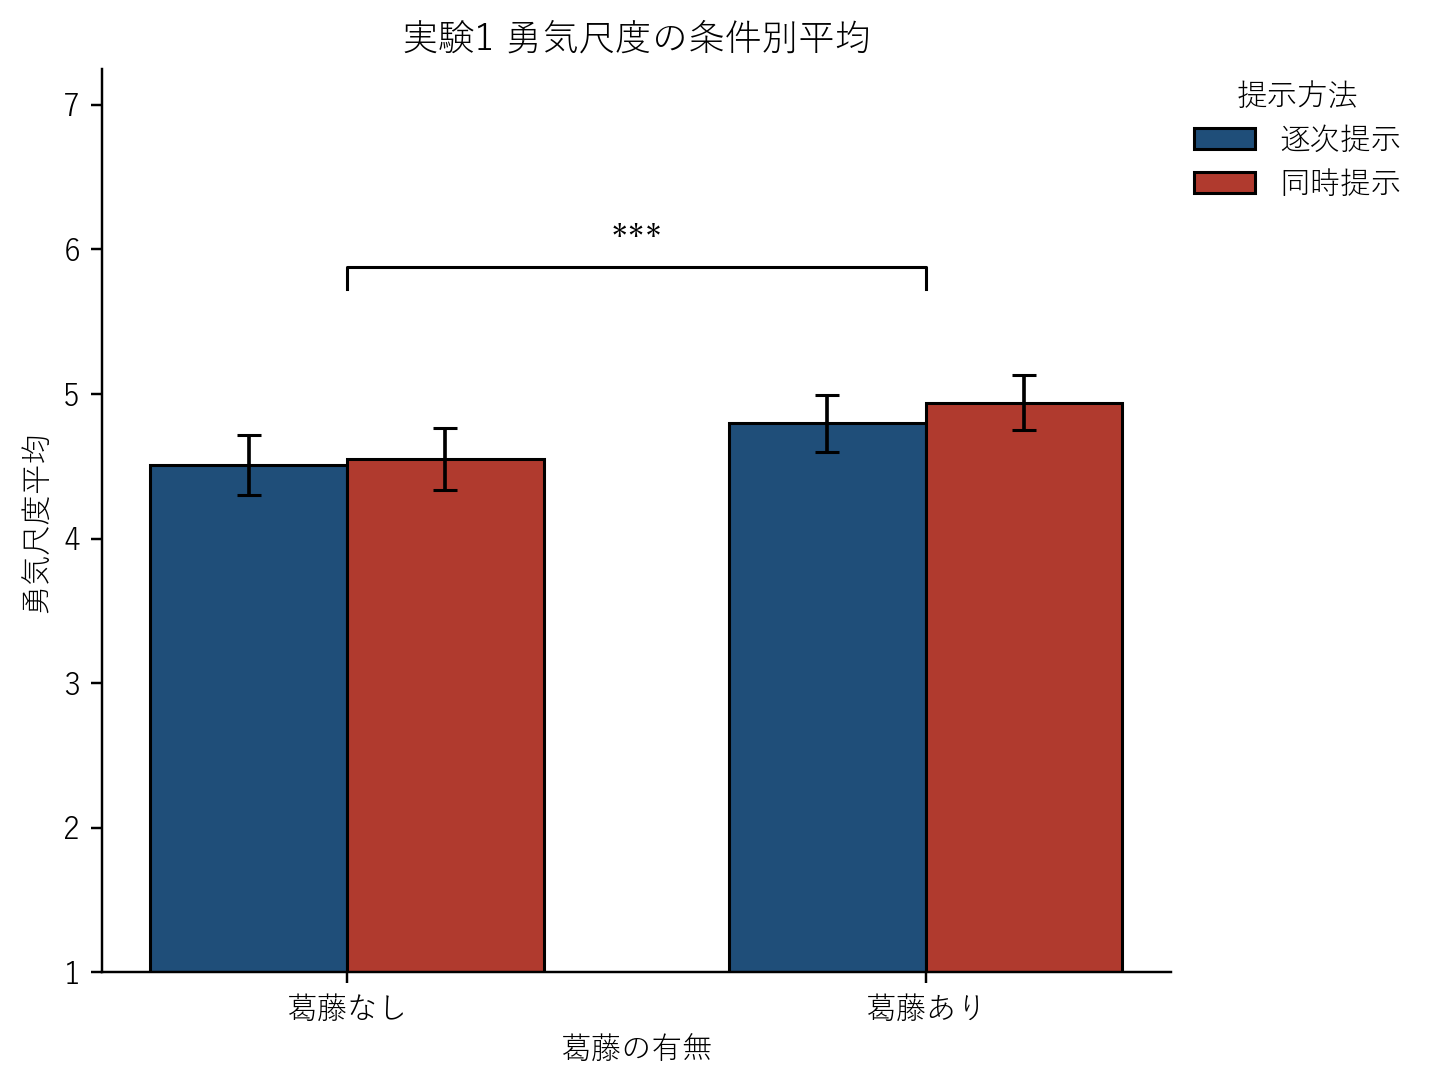
\includegraphics[width=0.86\linewidth]{fig3_study1_courage.png}
\caption{Condition means of courage ratings in Study 1.}
\label{fig:study1_courage}
\end{figure}

For conflict ratings, the conflict condition was rated higher than the no-conflict condition, and simultaneous presentation was rated higher than sequential presentation. The main effect of conflict was significant (F(1, 130) = 79.558, p \textless{} .001, generalized eta squared = .170). The main effect of presentation method was also significant (F(1, 130) = 46.448, p \textless{} .001, generalized eta squared = .039), and the interaction was significant (F(1, 130) = 4.924, p = .028). Condition means are shown in Figure~\ref{fig:study1_conflict}.

\begin{figure}[htbp]
\centering

\includegraphics[width=0.86\linewidth]{fig4_study1_conflict.png}
\caption{Condition means of conflict ratings in Study 1.}
\label{fig:study1_conflict}
\end{figure}

\subsection{Discussion}

In Study 1, the robot expressing approach-avoidance conflict was rated as more courageous than the robot in the no-conflict condition. This indicates that even when the behavior itself is the same, showing conflict between approach and avoidance motives before action makes the behavior easier to understand as involving fear or difficulty for the actor. This interpretation is consistent with the view that highly personal courageous actions involve fear or difficulty \citep{pury2007}. Therefore, externalizing internal states before action related to personal courage may be effective for presenting the robot's behavior as courageous to observers.

Conflict ratings were also higher in the conflict condition than in the no-conflict condition. This indicates that the presentation of approach and avoidance motives through speech bubbles was perceived by observers as approach-avoidance conflict. Regarding presentation method, no difference was found between sequential and simultaneous presentation in courage ratings. In contrast, conflict ratings were higher for simultaneous presentation. Therefore, simultaneous presentation was judged appropriate for Study 2 not as a method that makes the robot appear more courageous, but as a method that conveys conflict more clearly.

Study 1 confirmed that a robot expressing approach-avoidance conflict is perceived as courageous and provided evidence supporting the validity of the presentation to be used in Study 2. Based on these findings, Study 2 used the simultaneous presentation selected in Study 1 to examine the main purpose of the present research: whether observing a robot perceived as courageous affects observers' self-evaluations of personal courage.

\section{Study 2: Does Observing a Robot Perceived as Courageous Influence Observers' Self-Evaluations of Personal Courage?}

\subsection{Purpose}

The purpose of Study 2 was to examine how observing the robot confirmed in Study 1 to be perceived as courageous influences observers' self-evaluations of personal courage. We also examined whether this influence differs depending on observers' pre-existing courage tendency.

In Study 2, the presence or absence of conflict and the presence or absence of action were manipulated separately. This was because courage is understood as moving toward a valued action in a situation involving fear or difficulty \citep{rachman1984,woodard2007,norton2009}. In Chowkase et al.'s model as well, courage is described as a sequential process involving situation perception, value evaluation, evaluation of action feasibility, and action decision \citep{chowkase2024}. A condition showing only approach-avoidance conflict may reveal the observational effect of the internal state before action, whereas a condition showing only action may be limited to the observational effect of seeing the choice to move toward a valued action. Therefore, we separated the presence or absence of conflict and the presence or absence of action to distinguish among the effects of approach-avoidance conflict alone, action alone, and the combination of both.

In Study 2, we predicted that the effects of approach-avoidance conflict and action on observers' self-evaluations of personal courage would differ depending on pre-existing courage tendency. In particular, we predicted that, among participants with low pre-existing courage tendency, post-observation self-evaluation scores of personal courage would be highest in the conflict-with-action condition. The rationale was that the low-courage group, whose self-evaluations of courage were low, would be a group that experiences difficulty acting in conflict situations. Prior research has shown that observing a model who gradually copes while showing difficulty can increase self-efficacy and task performance \citep{schunk1987,schunk1989}. It has also been shown that when a task is difficult, people are more likely to use others' judgments and behavior as cues, whereas people with high self-efficacy are relatively independent from social influence \citep{lucas2006}. The conflict-with-action condition presents both the coexistence of avoidance and approach motives and the choice to move toward action. In other words, it presents a process that is close to the difficulty faced by the low-courage group while showing that this difficulty can be overcome. Therefore, we predicted that post-observation self-evaluation scores of personal courage would be highest in the low-courage group in this condition.

\subsection{Method}

\subsubsection{Conditions}

Study 2 used a three-factor mixed design with pre-existing courage tendency group as a between-participant factor and conflict and action as within-participant factors. Participants were classified into low- and high-courage groups based on their CM-J scores before stimulus presentation. Conflict was manipulated by whether both approach and avoidance motives were shown simultaneously or only one type of motive was shown. Action was manipulated by whether the robot produced the admonishing speech.

As in Study 1, the stimulus videos presented a scene in which the robot sees a person littering in a park. After showing situation recognition, the robot presented approach and avoidance motives in the speech bubble according to the condition. In the conflict condition, approach and avoidance motives were presented simultaneously and alternately enlarged and reduced. In the no-conflict, action-present condition, only approach motives were presented. In the no-conflict, action-absent condition, only avoidance motives were presented.

In the action-present condition, after the motive presentation, the robot said, ``Excuse me, this is not a place to throw away trash.'' In the action-absent condition, after the motive presentation, the robot did not speak, and a state in which it did not perform the admonishing behavior was presented.

\begin{table}[htbp]
\centering
\scriptsize
\caption{Study 2 conditions.}
\label{tab:study2_conditions}
\begin{tabularx}{\linewidth}{Y Y Y Y Y}
\toprule
Study 2 condition & Internal-state content & Motive statements used & Presentation method & Final admonishing speech \\
\midrule
No conflict, no action & Avoidance motives only & Avoidance motives: ``I would hate it if they yelled at me after I warned them''; ``Even if I warn them, they might ignore me and not take me seriously'' & Avoidance motives presented and emphasized & Absent \\
No conflict, action & Approach motives only & Approach motives: ``If I warn them, the park might become cleaner''; ``If I warn them, it might prompt that person to stop littering'' & Approach motives presented and emphasized & Present \\
Conflict, no action & Approach and avoidance motives & Approach motives: ``If I warn them, the park might become cleaner''; ``If I warn them, it might prompt that person to stop littering'' / Avoidance motives: ``I would hate it if they yelled at me after I warned them''; ``Even if I warn them, they might ignore me and not take me seriously'' & Simultaneous presentation with alternating emphasis & Absent \\
Conflict, action & Approach and avoidance motives & Approach motives: ``If I warn them, the park might become cleaner''; ``If I warn them, it might prompt that person to stop littering'' / Avoidance motives: ``I would hate it if they yelled at me after I warned them''; ``Even if I warn them, they might ignore me and not take me seriously'' & Simultaneous presentation with alternating emphasis & Present \\
\bottomrule
\end{tabularx}
\end{table}

\subsubsection{Measurement}

In Study 2, we measured pre-stimulus personal courage tendency, post-stimulus self-evaluations of the observer's own personal courage, and robot conflict ratings. All ratings were made on a 7-point scale. Personal courage was measured using the six items of the Japanese version of the Courage Measure (CM-J) \citep{shimotsukasa2023}. The CM-J is positioned as a scale that measures the trait and individual differences of courage to act despite fear or anxiety \citep{shimotsukasa2023}. In Study 2, the pre-stimulus CM-J score was used as an index of observers' pre-existing courage tendency. In contrast, the post-stimulus CM-J score was treated not as a change in long-term courage trait itself but as the observer's self-evaluation of personal courage immediately after stimulus presentation. In the analysis, the mean of the six items was used as the personal courage self-evaluation score.

Conflict ratings used the same four items as in Study 1. In the analysis, the mean of the four items was used as the conflict rating score. In addition, to confirm whether conflict ratings based on these four items corresponded to a direct judgment of conflict, the same direct item used in Study 1, ``This robot appeared to be experiencing conflict,'' was also obtained.

\subsubsection{Procedure}

Study 2 was conducted on Yahoo! Crowdsourcing. Participants first responded to the CM-J before stimulus presentation. They then viewed videos from the four conditions and, after each video, responded to self-evaluation items for their own personal courage and to robot conflict-rating items. The order of video presentation was fixed. This was done so that each participant could observe condition differences within the same context and more easily compare differences due to the presence or absence of approach-avoidance conflict and action within a single flow. The response data included video-content comprehension checks and attention-check items.

\subsubsection{Participants}

As in Study 1, exclusions were made based on video-content comprehension checks and attention-check items, resulting in a final analytic sample of 126 participants. Participants were 18 to 29 years old, with a mean age of 24.11 years (SD = 3.62). The sample included 55 men and 71 women. Based on pre-stimulus CM-J scores, participants with scores below 4 were classified as the low-courage group, and participants with scores of 4 or higher were classified as the high-courage group. The low-courage group included 69 participants, and the high-courage group included 57 participants.

\subsubsection{Statistical Analysis}

In Study 2, post-stimulus personal courage self-evaluation scores were analyzed as the main outcome, and conflict rating scores were analyzed as a manipulation check. For personal courage self-evaluation scores, a three-factor mixed analysis of variance was conducted with pre-existing courage tendency group based on pre-stimulus CM-J scores (below 4 vs. 4 or higher) as a between-participant factor and conflict (no conflict vs. conflict) and action (no action vs. action) as within-participant factors. Partial eta squared was reported as the effect size. When interactions were significant, simple effects were examined as needed. For simple-effects tests, normality of paired differences was examined using the Shapiro-Wilk test; paired t-tests were used when normality was satisfied, and Wilcoxon signed-rank tests were used when normality was not satisfied. Conflict rating scores were analyzed using the same factor structure to confirm the success of the conflict manipulation. Analyses were conducted using Python packages pandas, statsmodels, and SciPy.

\subsection{Results}

For observers' self-evaluations of personal courage, the hypothesized high score in the conflict-with-action condition among the low-courage group was not supported. However, the interaction between pre-existing courage tendency group and approach-avoidance conflict was significant (F(1, 124) = 7.513, p = .007, partial eta squared = .057).

Simple-effects analyses showed that, in the low pre-existing courage group, post-observation personal courage self-evaluation scores tended to be higher in the conflict condition (conflict M = 3.104, no conflict M = 2.982, t = 1.980, p = .052, d = .238). In contrast, in the high pre-existing courage group, post-observation personal courage self-evaluation scores were significantly lower in the conflict condition (conflict M = 4.757, no conflict M = 4.858, W = 404.0, p = .038, d = -.271).

The presence or absence of action did not show a significant effect on post-observation personal courage self-evaluation scores. Therefore, whether the robot actually performed the admonishing behavior did not have a clear additional effect on observers' self-evaluations of personal courage. This simple effect is shown in Figure~\ref{fig:study2_courage}.

\begin{figure}[htbp]
\centering

\includegraphics[width=0.86\linewidth]{fig5_study2_courage.png}
\caption{Simple effects of personal courage self-evaluations in Study 2. Means for the no-conflict and conflict conditions by pre-existing courage tendency group. Dagger indicates a marginal tendency; asterisk indicates a significant difference.}
\label{fig:study2_courage}
\end{figure}

As a manipulation check, conflict ratings were higher in the conflict condition than in the no-conflict condition. The main effect of conflict was significant (F(1, 124) = 52.939, p \textless{} .001, partial eta squared = .299). A supplemental check also showed that the conflict condition was rated higher than the no-conflict condition (W = 1128.0, p \textless{} .001, conflict M = 5.151, no conflict M = 4.209). Therefore, the conflict manipulation was successful in Study 2 as well.

\subsection{Discussion}

In Study 2, the hypothesis that the low-courage group would show the highest personal courage self-evaluation scores in the conflict-with-action condition was not supported. In addition, the presence or absence of action did not show a significant effect. Therefore, whether the robot actually performed the admonishing behavior itself cannot be said to have determined observers' self-evaluations of personal courage.

However, the interaction between pre-existing courage tendency group and approach-avoidance conflict was significant. This result indicates that presenting approach-avoidance conflict does not uniformly encourage observers but may operate in opposite directions depending on observers' pre-existing courage tendency. In the low-courage group, personal courage self-evaluation scores tended to be higher in the conflict condition. Previous studies have shown that observing a model who gradually copes while displaying difficulty can, in some circumstances, enhance self-efficacy and task performance more than observing a model who succeeds easily from the outset \citep{schunk1987,schunk1989}. Other work has shown that people are more likely to use others' judgments and behavior as cues when a task is difficult, whereas those with high self-efficacy are less susceptible to such influence \citep{lucas2006}. The conflict condition in the present study showed a process in which the robot held an approach motive despite also having an avoidance motive. For the low-courage group, this may have served as a cue that a motive to move toward valued action can coexist with fear or hesitation. However, pre-existing courage tendency and self-efficacy are not identical constructs, and we did not measure whether participants perceived the robot as a model coping with difficulty. Moreover, because this result was only marginal, this interpretation should remain tentative.

In contrast, in the high-courage group, personal courage self-evaluation scores were lower in the conflict condition. The high-courage group is a group with relatively high self-evaluation of moving toward valued action even in situations involving fear or difficulty. Therefore, even the same presentation of approach-avoidance conflict may have functioned for the high-courage group not as a supportive cue close to themselves but as information that made avoidance motives or the difficulty of the action salient. This interpretation is consistent with findings showing that robot interventions can change risk behavior and that, in uncertain tasks, participants tend to conform to a robot's judgment at an early stage \citep{hanoch2021,zonca2023}. In other words, the presentation of approach-avoidance conflict may have supported self-evaluation in the low-courage group but lowered self-evaluation in the high-courage group.

However, this study did not measure the extent to which observers perceived the robot as a model related to themselves, nor the extent to which they interpreted the robot's avoidance motives as information indicating the difficulty of the action. Therefore, the above interpretation remains a possibility.

\section{Limitations}

This study has several limitations. First, although this study measured observers' self-evaluations of personal courage, it did not measure whether observers actually moved toward valued action. The CM-J is positioned as a scale that measures the trait and individual differences of courage \citep{shimotsukasa2023}. Therefore, the post-stimulus CM-J score in this study should be interpreted not as a change in long-term courage trait but as observers' self-evaluations of personal courage immediately after stimulus presentation.

Second, this study did not directly measure the psychological process through which the presentation of approach-avoidance conflict operated in different directions for the low- and high-courage groups. In this manuscript, we suggested that for the low-courage group, the presentation may have served as a cue that ``a motive to move toward valued action can coexist with fear or hesitation,'' whereas for the high-courage group, it may have made avoidance motives or the difficulty of action more salient. However, because we did not directly measure whether the robot was perceived as a model coping with difficulty, perceived similarity to the robot, self-efficacy, interpretation of avoidance motives, perceived action difficulty, or reception of risk information, these remain interpretations.

Third, this study used only video stimuli involving a robot and did not compare other presentation media such as a physical robot, human model, avatar, animation, or text presentation. Therefore, it is not possible to separate whether the present results derive from the use of a nonhuman agent as a robot, from presenting the stimulus as a video, or from explicitly presenting approach-avoidance conflict through a speech bubble.

Fourth, in Study 2, the order of video presentation was fixed. Therefore, the results of Study 2 may include not only the effects of approach-avoidance conflict and action but also the influence of videos viewed previously and order effects. Future studies should use a counterbalanced presentation order to examine whether the same effect is replicated.

Fifth, the stimulus scenario in this study was limited to admonishing littering in a park. This scenario has some validity as a stimulus for examining personal courage because valued action and interpersonal risk coexist. However, the present study dealt with a scene in which the robot directly admonished a stranger's norm violation. Personal courage may include diverse situations such as speaking up in interpersonal contexts, seeking help, challenging learning tasks, social reintegration, and prosocial behavior \citep{pury2007,howard2017,vogel2007}. Therefore, it remains unclear whether the present findings generalize to situations involving different types of risk or action value.

\section{Future Work}

Future research should proceed in two directions: basic and applied approaches. In the basic approach, it is necessary to examine the psychological process through which presenting approach-avoidance conflict affects observers' self-evaluations of personal courage. Specifically, future studies should measure the extent to which observers perceive the robot as a self-relevant model or as a model coping with difficulty, perceived similarity to the robot, self-efficacy, perceived threat and difficulty, and the added value of action information, and clarify the conditions under which the interaction between pre-existing courage tendency and approach-avoidance conflict emerges. In addition, using the same scenario and internal-state expression, future work should compare a robot present in front of the observer, a robot in a video, a human model, avatars or animations, and text presentation, and examine the conditions under which a nonhuman robot functions as a social model as well as the roles played by the robot's physical embodiment, co-presence, and movement.

In the applied approach, it is necessary to identify target populations and situations in which effects are expected and then examine them. In particular, for people with low pre-existing courage tendency, concrete support contexts may include challenging new learning tasks in educational settings, building interpersonal relationships in counseling or social reintegration contexts, and everyday prosocial behavior. In such contexts, future studies should measure not only post-observation self-evaluation but also actual action choices, such as speaking up, asking questions, seeking help, pointing out problems, and helping others, as well as sustained changes in these behaviors.

\section{Conclusion}

This study examined the possibility that a robot, as a nonhuman agent, can influence observers' self-evaluations of personal courage by externalizing and presenting an internal state before action, namely approach-avoidance conflict. Study 1 confirmed that a robot expressing approach-avoidance conflict is perceived as courageous. Study 2 showed that observing such a robot does not uniformly influence observers' self-evaluations of personal courage but may relate to them differently depending on pre-existing courage tendency. These results do not demonstrate an effect unique to robots, but they indicate the possibility of using robots as social models that present internal states before action.

\section*{Conflict of Interest Statement}
The authors declare that the research was conducted in the absence of any commercial or financial relationships that could be construed as a potential conflict of interest.

\section*{Author Contributions}
YS was responsible for study design, stimulus creation, data analysis, and manuscript writing. MB, HT, and HI contributed to study design, interpretation of the results, and manuscript revision.

\section*{Funding}
Funding information for this study will be added before submission.

\section*{Acknowledgments}
The authors thank the people who provided advice during the conduct of this study.

\section*{Data Availability Statement}
The availability and sharing method of the data analyzed in this study will be added before submission.

\bibliographystyle{Frontiers-Harvard}
\bibliography{references_japanese}

\end{document}
